\documentclass{ecai}
\usepackage{times}
\usepackage{graphicx}
\usepackage{latexsym}
\usepackage{hyperref}
\usepackage{paralist}
%\usepackage{enumitem}
\usepackage{xcolor}
\usepackage{xspace}
\usepackage{amsmath}
% \usepackage{algpseudocode}
\usepackage[ruled,linesnumbered]{algorithm2e}


\newcommand\m[1]{\ensuremath{#1}\xspace}
\newcommand\ltrue{\m{\mathbf{t}}}
\newcommand\lunkn{\m{\mathbf{u}}}
\newcommand\lfalse{\m{\mathbf{f}}}
\newcommand\leqp{\m{\leq_p}}
\newcommand\geqp{\m{\geq_p}}
\newcommand\entails{\m{\models}}
% \newcommand\land{\m{\wedge}}
\newcommand\limplies{\m{\Rightarrow}}

% \SetKwInput{Input}{input} 

\newcommand\allconstraints{\m{T_P}}

%%\ecaisubmission   % inserts page numbers. Use only for submission of paper.
% Do NOT use for camera-ready version of paper.

\newcommand\bart[1]{{\color{red}\textsc{BB}: #1}}
\newcommand\tias[1]{{\color{green}\textsc{TG}: #1}}
\newcommand\emilio[1]{{\color{blue}\textsc{EG}: #1}}

%%\ecaisubmission   % inserts page numbers. Use only for submission of paper.
                  % Do NOT use for camera-ready version of paper.

\begin{document}

\title{Step-wise explanations of logic problems by automated reasoning}

\author{\{Bart, Emilio, Jens, Tias\}; 7 pages +1 with refs}

\maketitle


\begin{abstract}
We explore the problem of step-wise explaining how to solve logic problems, for example logic grid puzzle. The main challenge is that automated reasoning can freely combine all knowledge in its knowledge base to make derivations. In contrast, we want explanations to be simple and cognitively easy, so that a human can easily verify the reasoning step, and learn how to make similar reasoning steps.
We identify the problem as that of finding a good ordering of self-contained reasoning steps. Different interpretations of good ordering as well as self-containedness of a reasoning step are discussed. To make the search for a good ordering feasible in reasonable time, we propose an iterative refinement approach where minimal unsat core's over well-defined decompositions of the problem are searched. Our experiments show the feasibility of the approach in terms of the ordering and size of the explanations given as well as the computation time needed.
\end{abstract}

%The page limit for ECAI scientific papers is {\bf 7} pages, plus one ({\bf 1})

\section{Intro}



%Need for explanations of reasoning systems
In the last few years, as AI systems employ more advanced reasoning mechanisms and computation power, it becomes increasingly difficult to understand why certain decisions are made. 
Explainable AI (XAI) research aims to fulfil the need for trustworthy AI systems to understand why the system made a decision for verifying the correctness of the system, as well as to control for biased or systematically unfair decisions.

Explainable AI is often studied in the context of (black box) prediction systems such as neural networks, where the goal is to provide insight into what part of the input is important in the \textit{learned} model. 
These insights (or local approximations thereof) can justify why certain predictions are made.
In contrast, in Constraint Satisfaction Problems (CSP), the problem specification is an explicit model-based representation of the problem, hence creating the opportunity to explain the inference steps directly in terms of this representation.



% Explainable AI research aims to fulfil the need for trustworthy AI systems that can explain their reasoning in a human-understandable way. 
% As these systems employ more advanced reasoning mechanisms and computation power, it becomes increasingly difficult to understand why certain decisions are made. 
% Understanding the decisions is important for verifying the correctness of the system, as well as to control for biased or systematically unfair decisions.

% Explainable AI is often studied in the context of (black box) machine learning systems such as neural networks, where the goal is to provide insight into what part of the input is important in the \textit{learned} model. These insights (or local approximations thereof) can justify why certain predictions are made. In contrast, in constraint satisfaction problems, the problem specification is an explicit model-based representation of the problem, hence creating the opportunity to explain the inference steps directly in terms of this representation.

Explanations have been investigated in constraint solving before, most notably for explaining overconstrained, and hence unsatisfiable, problems to a user~\cite{junker2001quickxplain}.
Our case is more general in that it also works for satisfiable problems.
At the solving level, in lazy clause generation solvers, explanations of a constraint are studied in the form of an implication of low-level Boolean literals that encode the result of a propagation step of an individual constraint~\cite{feydy2009lazy}. 
Also, no-goods (learned clauses) in conflict-driven clause learning SAT solvers can be seen as explanations of failure during search~\cite{marques2009conflict}. 
These are not meant to be human-interpretable but rather to propagate efficiently.

We aim to explain the process of propagation in a constraint solver, independent of the consistency level of the propagation and without augmenting the propagators with explanation capabilities.
For problems that can --- given a strong enough propagation mechanism --- be solved without search, e.g. problems such as logic grid puzzles with a unique solution, this means explaining the entire problem solving process. 
For problems involving search, this means explaining the inference steps  in one search node. 
It deserves to be stressed that we are not interested in the computational cost of performing an expensive form of propagation, but in explaining all consequences of a given assignment to the user in a way that is as understandable as possible. 

More specifically, we aim to develop an explanation-producing system that is complete and interpretable. 
By \textit{complete} we mean that it finds a \textit{sequence} of small reasoning steps that, starting from the given problem specification and a partial solution, derives all consequences. 
Gilpin et al.~\cite{DBLP:conf/dsaa/GilpinBYBSK18} define \textit{interpretable} explanations as ``descriptions that are simple enough for a person to understand, using a vocabulary that is meaningful to the user''. 
Our guiding principle is that of simplicity, where smaller and simpler explanations are better. 
For those explanation steps that are still too complex, we provide a mechanism that allows \emph{zooming in} onto the explanation step and thus enables explanations at different levels of abstraction. Our nested explanation sequences are inspired by counterfactual reasoning, as often found in research on actual causality and by proofs by contradiction, as common in mathematics.

In practice, we choose to represent the constraints in natural language, which is an obvious choice for logic grid puzzles as they are given in the form of natural language \textit{clues}. 
We represent the previously and newly derived facts visually, as can be seen in the grid in Figure~\ref{fig:zebrascreen}, in which it is visualized that the implicit ``Bijectivity'' axiom present in each logic grid puzzle is used to derive that since Arrabiata sauce was eaten with Farfalle, it was not eaten with any of the other pasta types.

\bart{Make better quality screenshot! Also check the others. }
\begin{figure}[ht]
\centering
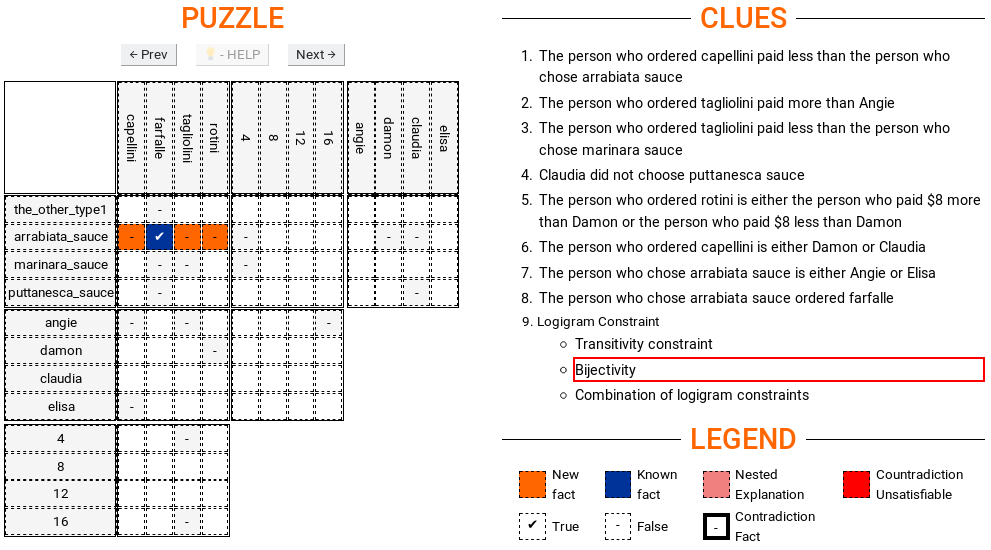
\includegraphics[width=\linewidth]{figures/zebra_screen_1}
\caption{Demonstration of explanation visualisation.}
\label{fig:zebrascreen}
\end{figure}

%HolyGrail challenge and related work
Our work is motivated by the ``Holy Grail Challenge''\footnote{\url{https://freuder.wordpress.com/pthg-19-the- third-workshop-on-progress-towards-the-holy-grail/}} which had as objective to provide \textit{automated} processing of logic grid puzzles, ranging from natural language processing, to solving, and explaining.
% An earlier version of our system won the challenge at the workshop. 
\emilio{do we really need to say that ?}\bart{What? The line in comment about winning above? Not really, no}
While the \ourtool, our integrated system, has the capability of solving logic grid puzzle starting from the natural language clues (see Section \ref{sec:holistic}), the focus of this contribution is on the explanation-producing part of the system.

The explanation-generating techniques we develop can be applied in a multitude of use cases. 
For instance, our tool can explain the entire sequence of reasoning, such that a user can debug the reasoning system or the set of constraints that specify their problem. 
As our approach starts from an arbitrary set of facts, it can also be used as a virtual assistant when a user is stuck in solving a problem.
The system will explain the simplest possible next move, or in an interactive setting, the system can explain how it would complete a partial solution of a user.
Finally, our measures of simplicity of reasoning steps can be used to estimate the difficulty of solving a problem for a human, e.g. for gradual training of experts.
\bart{Mention interactive configuration here as an application domain? }


Our main contributions are the following:
\begin{itemize}
	\item We formalize the problem of step-wise explaining the propagation of a constraint solver through a sequence of small inference steps;
	\item We propose an algorithm that is agnostic to the propagators and the consistency level used, and that can provide explanations for inference steps involving arbitrary combinations of constraints;
	\item Given a cost function quantifying human interpretability, our method uses an optimistic estimate of this function to guide the search to low-cost explanations, thereby making use of Minimal Unsatisfiable Subset extraction;
	\item We introduce nested-explanations to refine explanations of complex inference steps using counterfactual reasoning; \emilio{contrastive explanations ?}\bart{What about them? That is not really what this nested is...}
	\item We experimentally demonstrate the quality and feasibility of the approach in the domain of logic grid puzzles.
\end{itemize}


This paper is structured as follows. In Section~\ref{sec:related-work}, we discuss related work. Section \ref{sec:background}, explains the rules of logic grid puzzles and presents background information. 
Sections \ref{sec:problem-definition} and \ref{sec:nested-explanation}, formalize the theory of the explanation-production problem on multiple abstraction levels, while Section \ref{sec:expl-gen-prod} describes the algorithms needed to solve the explanation-production problem. 
In Section \ref{sec:zebra}, we motivate our design decisions using observations from the use case. 
Section \ref{sec:holistic} describes the entire pipeline of the \ourtool integrated system. 
In Section \ref{sec:experiments}, we experimentally study the feasibility of our approach. 
Finally, we conclude the paper in Section \ref{sec:conclusion}.


% Publication history
\paragraph*{Publication history} This paper is an extension of a couple of previous papers presented at workshops and conferences \cite{claesuser,DBLP:conf/bnaic/ClaesBCGG19,ecai/BogaertsGCG20}. The current paper extends the previous papers we more detailed examples, additional experiments, as well as a formal treatment of what we call \emph{nested explanation sequences} (an idea that first appeared in a demo we submitted to IJCAI-PRICAI 2020 but that is first formalized in the current paper).  

% Our nested explanation XAI submission stems from the work originally proposed \cite{ecai/BogaertsGCG20} and motivated by the results from the demonstrator submitted to IJCAI-PRICAI 2020.



\section{Related work}
This research fits within the general topic of Explainable Agency~\cite{langley2017explainable}, whereby in order for people to trust autonomous agents, the latter must be able to explain their decisions and the reasoning that produced their choices. 
For example, explainable planning~\cite{fox2017explainable} is concerned with building planning systems that can explain their own behaviour. This includes answering queries such as ``why did the system (not) make a certain decision?'', ``why is this the best decision?'', etc. In contrast to explainable machine learning research, in explainable planning one can make use of the explicit \textit{model-based representation} over which the reasoning happens. Likewise, we will make use of the constraint specification available to constraint solvers. 

Explanation of Constraint Satisfaction Problems (CSP) has been studied mostly in the context of overconstrained problems. 
The goal then is to find which constraints conflict with each other. The QuickXplain method \cite{junker2001quickxplain} for example uses a dichotomic approach that recursively partitions the constraints to find a minimal conflict set. This is also known as the Minimum Unsat Subset (MUS) problem or Minimal Unsat Core extraction~\cite{marques2010minimal}. Many algorithm exist for finding a MUS or enumerating all MUS's~\cite{marques2010minimal}. We will use MUS extraction for finding a minimal explanation of an individual inference step.

Our work is inspired by the holy grail challenge at CP'2019, which in turn has its roots in earlier work of E.~Freuder on inference-based explanations \cite{sqalli1996inference}. In that work, the authors investigate logic grid puzzles and develop a number of problem-specific inference rules that allow solving such puzzles without search. These inference rules are equipped with explanation templates such that each propagation event of an inference rule also has a templated explanation, and hence an explanation of the solution process is obtained. We point out that the more complex inference rules (NCC and GNCC) are in inference rules over hard-coded combinations of (in)equality constraints. In contrast, our proposed method works for any type of constraint and any combination of constraints, and automatically infers a minimal set of facts and constraints that explain an inference step, without using any problem-specific knowledge.

There is a rich literature on automated and interactive theorem proving, recently focussing on providing proofs that are understandable for humans \cite{Ganesalingam2017} and, e.g.,  on teaching humans -- using interaction with theorem provers -- how to craft mathematical proofs  \cite{DBLP:conf/icml/YangD19}. 
Our work fits into this line of research since our generated explanations can also be seen as proofs, but in the setting of finite-domain constraint solving.

Our approach also relates to the work of Belahcene et.\ al.~\cite{belahcene2017explaining} who --- in the context of decision-aiding --- aim to build incremental explanations using preference relations. In our case, this would correspond to preferring simple constraints to more complex combinations of constraints through a cost function.

\section{Background}

\paragraph{Logic grid puzzles}
Our proposed method is applicable to constraint satisfaction problem \tias{with a unique solution?}. We will use \textit{logic grid puzzles} as example domain, as it requires no expert knowledge to understand.

A logic grid puzzle (also known as a Zebra puzzle or Einstein puzzle) consists of a set of natural language sentences (from hereon referred to as ``clues'') and (optionally) a set of \emph{entities} occurring in those sentences. 
For instance, our running example contains a clue ``The person who chose arrabiata sauce is either Angie or Elisa'' and (among others) entities ``arrabiata sauce'', ``Angie'' and ``Elisa''. 

The set of entities is sometimes left implicit if it can be derived from the clues, but often it is given in the form of a grid. Furthermore, in such a puzzle the set of entities is partitioned into equally sized groups (corresponding to \emph{types}); in our example, at least ``person'' and ``sauce'' are such types. 

The goal of the puzzle is to find relations between each two types such that
\begin{compactitem}
	\item each clue is respected, 
	\item each entity of one type is matched with exactly one entity of the second type, e.g., each person chose exactly one sauce (this type of constraint will be referred to as \emph{bijectivity}), and 
	\item the relations are logically linked, e.g., if Angie chose arrabiata sauce and arrabiata sauce was paired with farfalle, then Angie must also have eaten farfalle (from now on called \emph{transitivity}). 
\end{compactitem}
In section Sec~\ref{sec:holistic} we explain how we obtain a vocabulary and first-order theory in a mostly automated way from the clues. The result is a vocabulary with types corresponding to the groups of entities in the clues, and the names and types of the binary relations to find (e.g \textit{chose(person, sauce)}, \textit{paired(sauce, pasta)}, \textit{eaten(person, pasta)});
%We furthermore assume that the interpretation of the types is fixed (and hence all interpretations agree on this). 
as well as first-order sentences corresponding to the clues, and the bijectivity and transitivity constraints. Let $T_P$ be a theory containing all of these sentences for a given puzzle $P$.

Our running example is a puzzle about people having dinner in a restaurant and ordering different types of pasta. It is the harderst logic grid puzzle we encountered (as a reference, at a recent AI conference, when presenting our tool \cite{DBLP:conf/bnaic/ClaesBCGG19}, only four out of 80 researchers who tried managed to solve it).    
The entire puzzle can be seen in Figure \ref{fig:zebrascreen}; the full final explanation generated for it can be found at \url{http://bartbog.github.io/zebra/pasta}.
% Dout of  and its final produced explanation still contains some challenging steps. 

\paragraph{Typed first-order logic}
Our reasoning method is based on \emph{typed first-order logic}. %, with links to \emph{typed second-order logic}.
Part of the input is a logical vocabulary consisting of a set of type symbols, typed constant symbols, and relation symbols with associated type signature (i.e., each relation symbol is typed $T_1\times \dots \times T_n$ with $T_i$ types).\footnote{We here omit function symbols since they are not used in this paper.} For example, type \textit{person} with constant symbol \textit{Angie} of type \textit{person} and a relation \textit{choseSauce(.,.)} with signature \textit{person $\times$ sauce}.


A \emph{first-order theory} is a set of sentences (well-formed variable-free first-order formulas in which each quantified variable has an associated type). 
Given a logical vocabulary $V$, a \emph{\textbf{partial} interpretation} $I$ assigns to each type symbol $T$ (e.g. \textit{person}) a finite set $I(T)$ and to each 
relation symbol $P$ with type signature $T_1\times \dots \times T_n$ a function 
\[I(P): I(T_1)\times \dots \times I(T_n)\to \{\ltrue,\lunkn,\lfalse\},\] 
where $\ltrue$ stands for true, $\lunkn$ for unknown, and $\lfalse$ for false. In case all functions $I(P)$ map all tuples into $\{\ltrue,\lfalse\}$ (i.e., no more tuples are unknown), we call $I$ a \emph{full interpretation} (this is sometimes also called a \emph{total} or \emph{two-valued} interpretation, or simply \emph{an interpretation}). 
A partial interpretation $I_1$ is \emph{more precise} than partial interpretation $I_2$ (notation $I_1\geqp I_2$) if $I_1$ and $I_2$ agree on everything not unknown in $I_2$.

% 
% In a second-order theory also quantifiers over relations have an associated type signature. 
% \bart{Clear or do I make it more formal}
% 
% \bart{There might be some related work in interactive theorem proving. If the system proposes a ``simple'' proof of a theorem... Very similar to what we do here.}


\section{Problem definition}
A logic grid puzzle  (also known as a Zebra puzzle or Einstein puzzle after Einstein's famous example of this type of puzzle) consists of a set of natural language sentences (from hereon referred to as ``clues'') and (optionally) a set of \emph{entities} occurring in those sentences. 
For instance, our running example contains a clue ``The person who chose arrabiata sauce is either Angie or Elisa'' and (among others) entities ``arrabiata sauce'', ``Angie'' and ``Elisa''. 
The set of entities is sometimes left implicit if it can be derived from the clues, but often it is given in the form of a grid. 
Furthermore, in such a puzzle the set of entities is partitioned into equally sized groups (corresponding to \emph{types}); in our example, at least ``person'' and ``sauce'' are such types. 
The goal of the puzzle is to find relations between each two types such that
\begin{compactitem}
	\item each clue is respected, 
	\item each object of one type is linked to exactly one object of the second type, e.g., each person ordered exactly one sauce (this type of constraint will be referred to as \emph{bijectivity}), and 
	\item the relations are logically linked, e.g., if Angie ordered arrabiata sauce and arrabiata sauce was paired with farfalle, then Angie must also have eaten farfalle (from now on called \emph{transitivity}). 
\end{compactitem}

For now, we assume that a vocabulary with types corresponding to the groups of entities in the clues and binary relations between each two types is given.
We furthermore assume that the interpretation of the types is fixed (and hence all interpretations agree on this). 
Finally, we assume that the clues, as well as the bijectivity and transitivity constraints are given as first-order sentences and that $T_P$ is a theory containing all of these sentences for a given puzzle $P$; we discuss how to obtain this logical form in Section \ref{sec:holistic}.
When a human solves a logic grid puzzle, they typically maintain a grid with all the information obtained so far and use it in combination with the clues to derive new conclusions. In logic terminology, the user maintains a partial interpretation.  
With this in min, the goal underlying our tool is to find a sequence of partial interpretations of the involved relations (e.g., in which it is known that Angie did not choose arrabiata sauce, but it still unknown whether she ordered farfalle) with a 
\emph{justification} (see below) of why each of the steps is correct that is ``as easy to understand as possible''. 
Of course the latter is a subjective matter and quite hard to quantify. Therefore, in this paper, we will use a reasonable approximation thereof. 


\paragraph{Justification of Reasoning Steps.}
As mentioned above, we are searching for a sequence 
\[ I_0 = \emptyset, I_1 = I_0 \cup N_1, \dots , I_n = I_{n-1}\cup N_n\]
where $I_i$ represents the state of the grid at each point in time and $N_i$ represents the newly derived information. 
Furthermore, it is important that each reasoning step be accompanied with a \emph{justification}. By that we mean a tuple $(E_i,S_i)$ such that: 
\begin{compactitem}
	\item $E_i\subseteq I_i$ (i.e., the explaining facts are a subset of what was previously derived),
	\item $S_i \subseteq T_P$ (i.e., only some of the clues and implicit constraints are used), and 
	\item $S_i \cup E_i \entails N_i$ (i.e., all newly derived information indeed follows from this justification).
\end{compactitem}
A first observation related to this definition is that it nowhere specifies \emph{quality} of the justifications, this manifests at least in two forms already. First of all, any superset of a justification is a justification itself (it seems clear that a bare minimal demand on our justifications should be that they are subset-minimal), and secondly, since since logic grid puzzles have a unique solution, say $Sol$ the sequence 
\[I_0, Sol\]
with justification $(\emptyset,T_P)$ always satisfies this definition. That justification simply states ``this is the solution because, well, it is'' and is of course extremely uninformative. However, the current definition only establishes what constitutes a correct justification, quality of justifications is studied later on. 

Another observation is that the problem checking whether $(E_i,S_i)$ explains $N_i$ is definitely in co-NP since this problem can be performed by verifying that $S_i \land \lnot N_i$ has no models more precise than $E_i$ and hence is an instance of the negation of a model expansion problem \cite{ternovskaMXcomplexity}. 
Furthermore, the task of finding a \emph{subset-minimal} justification can easily be cast, after reifying the involved constraints as a second-order problem of the form
\[\exists S_i\subseteq T_P, E_i\subseteq I_i: (\forall I: I\models S_i\land E_i \Rightarrow N_i) \land \lnot \exists S_i'\subseteq S_i, E_i'\subseteq E_i: \forall ... \]
\bart{Not sure how valuable it is to put this here.}
In principle our problem of finding subset-minimal (or even, see the next paragarph, cost-optimal) justifications could be solved by specifying it in such a way in second-order logic and subsequently finding models for it, e.g. by a reduction to QBF \cite{kr/BogaertsTS16,kr/vanderHallenJ18}. 
However, since this is already an $\exists\forall\exists SO$ specification, we expect this approach not be feasible (this expectation remains to be verified in future work). 



\paragraph{Simplicity of reasoning steps.}
While subset-minimality appears to be a necessary condition for acceptable justifications, it certainly is not a sufficient condition. 
Indeed, at a certain point in the explanation sequence, many different subset-minimal justifications can exist and not all of them are equally simple. 
Compare for instance using a single clue to derive a new fact with using the combination of two clues and five previously derived facts to find a new fact. 
To approximate of how easy to understand a justification is (i.e., a single transition in the above described sequence), we start from the simple cognitive idea \bart{can we cite this somewhere? } that (in general) the fewer things a human needs to have in memory simultaneously, the easier the task at hand is. 
Hence, as a measure of difficulty we propose to use a weight function in terms of \textbf{the total number of clues, bijectivity and transitivity constraints, and previously derived facts} needed to derive a new fact. \bart{In fact ,we do not exactly use this measure, since we do not allow combining two clues if there exists some explanation that only uses one}
The reader should be advised that this is quite a rough approximation; for instance certain clues can be easier than others to reason about (e.g., compare ``Claudia did not choose puttanesca sauce'' with ``The person who ordered rotini is either the person who paid \$8 more than Damon or the person who paid \$8 less than Damon'') or it might be that humans perceive reasoning about clues in general as easier or harder than reasoning about the implicit (bijectivity and transitivity) constraints presents in logic grid puzzles. While researching better measures is an interesting topic, it falls out of the scope of the current paper. Moreover, many ideas of the current work remain valid when the actual measure is changed. 
Our observatoin from below, that using second-order logic tools such as e.g. \cite{proB,kr/BogaertsTS16} to find cost-optimal justifications is an option remains valid as long as the cost-functoin is expressible in (a sufficient extension of SO). Yet, due the high complexity, is not a direction we explored. 
\bart{Actually, I would really like to try this sometimes. The complexity argument is valid. But since we have small domains it is actually not so relevant... Maybe it works well. In that case it would yield good explanations!  }


\paragraph{Simple sequence vs simple steps}
In the above, we focused on generating and defining understandability of a single step in the reasoning process. 
However, in its most general form, we would like to optimize the understandability of the entire sequence of explanations. 
For this, even defining a measure seems to be a very hard task (for instance, is the understandability of a sequence related to its most difficult step or to its average difficulty? Sometimes even the ordering of the steps might make a difference for humans, even though the actual steps are the same, ...). 
Furthermore, even if we fix a measure, the problem of holistically optimizing a sequence of explanation steps is much harder than optimizing a single step since there are exponentially more sequences. 
Therefore, in the current paper, we take a greedy approach where at each step, the best next possible explanation is chosen, without taking global optimality of the sequence in mind. The results we obtain this way are satisfying. 



% The grand goal underlying our tool is to find, given a logic grid puzzle (of which we assume it is given in some logical form for now; we revisit this in Section \ref{sec:holistic}), to find a sequence of partial assignments of variables (e.g., where it is already determined that certain entities are linked (or not linked) to which other entities) that is ``as easy to understand'' as possible.  
% Of course the latter is quite a vague concept and hard to find an objective measure for. However, we 
% The larger problem




\section{Explanation-producing search}\label{sec:expl-gen-prod}
In this section, we tackle the goal of searching for a non-redundant explanation sequence that is as simple as possible to understand.

Ideally, we could generate all explanations of each fact in $max(I_0,\allconstraints)$, and search for the lowest scoring sequence among those explanations. However, the number of explanations for each fact quickly explodes with the number of constraints, and is hence not feasible to compute. Instead, we will iteratively construct the sequence, by generating candidates for a given partial interpretation and searching for the smallest one among those.

\myparagraph{Sequence construction}
We aim to minimize the cost of the explanations of the sequence, measured with an aggregate over individual explanation costs $f(E_i, S_i, N_i)$ for some aggregate like $max()$ or $average()$. The cost function $f$ could for example be a weighted sum of the cardinalities of $E_i$, $S_i$ and $N_i$; in Section~\ref{sec:cost}, we discuss a concrete cost function for the use case of logic grid puzzles.

Instead of globally optimizing the aggregated sequence cost, we encode the knowledge that we are seeking a sequence of small explanations in our algorithm. Namely, we will greedily and incrementally build the sequence, each time searching for the lowest scoring next explanation, given the current partial interpretation. Such an explanation always exists since the end point of the explanation process $max(I_0,\allconstraints)$ only contains consequences of $I_0$ and \allconstraints.

Algorithm \ref{alg:main} formalizes the greedy construction of the sequence, which determines $I_{end} = max(I_0,\allconstraints)$  through propagation and relies on a \textit{min-explanation$(I,\allconstraints)$} function to find the next cost-minimal explanation.

\begin{algorithm}
	\DontPrintSemicolon
	  \Input{A initial interpretation $I_0$ and a set of constraints $\allconstraints$}
	  \Output{An explanation sequence $Seq$}
  %  \begin{algorithmic}
  $I_{end} \gets$ propagate$(I_0\land \allconstraints)$\;
  Seq $\gets$ empty sequence\;
  $I \gets I_0$\;
  \While{$I \neq I_{end}$}{
    $(E, S, N) \gets $min-explanation$(I, \allconstraints)$\;
    append $(E, S, N)$ to Seq\;
    $I \gets I \cup N$\;
  }
  % \end{algorithmic}
  \caption{High-level greedy sequence-generating algorithm.}
  \label{alg:main}
\end{algorithm}
\myparagraph{Candidate generation}
The main challenge is finding the lowest scoring explanation, among all reasoning steps that can be applied for a given partial interpretation $I$. We first study how to \textit{enumerate} a set of candidate non-redundant explanations given a set of constraints.

For a set of constraints $\allconstraints$, we can first use propagation to get the set of new facts that can be derived from a given partial interpretation $I$ and the constraints $\allconstraints$. 
%\emilio{why a ? and not n ? Vor visibility ?} -> you are right, 'n' is more consistent. Changing...
For each new fact $n$ not in $I$, we wish to find a non-redundant explanation $(E \subseteq I, S \subseteq \allconstraints,\{n\})$ that explains $n$ (and possibly explains more). 
Recall from Definition~\ref{def:nonred} that this means that whenever one of the facts in $E$ or constraints in $\allconstraints$ is removed, the result is no longer an explanation.
We now show that this task is equivalent to finding a Minimal Unsat Core (or Minimal Unsat Subset, MUS).
To see this, consider the theory
\[ I\wedge \allconstraints \wedge \lnot n.\]
This theory surely is unsatisfiable since $n$ is a consequence of $I$ and $\allconstraints$.
Furthermore, under the assumption that $I\wedge \allconstraints$ is consistent (if it were not, there would be nothing left to explain),
\emph{any} unsatisfiable subset of this theory contains $\lnot n$.
We then see that each unsatisifiable subset of this theory is of the form $E \wedge S \wedge \lnot n$ where $(E,S,\{n\})$ is a (not necessarily redundant) explanation of the derivation of $\{n\}$ from $I$.
Vice versa, each explanation of $\{n\}$ corresponds to an unsatisifiable subset. Thus, the \emph{minimal} unsatisifiable subsets (MUS) of the above theory are in one-to-one correspondence with the non-redundant explanations of $n$, allowing us to use existing MUS algorithms to search for non-redundant explanations.

We must point out that MUS algorithms typically find \textit{an} unsatisfiable core that is \textit{subset-minimal}, but not \textit{cardinality-minimal}. That is, the unsat core can not be reduced further, but there could be another minimal unsat core whose size is smaller.
That means that if size is taken as a measure of simplicity of explanations, we do not have the guarantee to find the optimal ones. And definitely, when a cost function kicks, optimality is also not guaranteed.

Algorithm~\ref{alg:cand} shows our proposed algorithm. The key part of the algorithm is on line \ref{line:mus} where we find an explanation of a single new fact $n$ by searching for a MUS that includes $\neg n$.
We search for subset-minimal unsat cores to avoid redundancy in the explanations.
Furthermore, once a good explanation $(E,S,N)$ is found, we immediately explain all implicants of $E$ and $S$. In other words: we take $N$ to be subset-maximal.
The reason is that we assume that all derivable facts that use the same part of the theory and the same part of the previously derived knowledge probably require similar types of reasoning and it is thus better to consider them at once.
Thus, we choose to generate candidate explanations at once for all implicants of $(E, S)$ on line~\ref{line:implicants}.
Note that the other implicants $N \setminus \{n\}$ may have simpler explanations that may be found later in the for loop, hence we do not remove them from $J$.

\begin{algorithm}
  % 
  \DontPrintSemicolon
  
  \SetKwComment{command}{/*}{*/}

  \Input{A partial interpretation $I$ and a set of constraints $\allconstraints$}
\Output{A set of candidate explanations $Candidates$}
  Candidates $\gets \{\}$\;
  $J \gets$ propagate$(I \wedge \allconstraints)$\;
  \For{$n \in J \setminus I$\label{line:for}}{
    \tcp{\small Minimal expl. of each new fact:}
    $X \gets MUS(\neg n \wedge I \wedge \allconstraints)$ \label{line:mus}\;
    $E \gets I \cap X$\tcp*{\small facts used}
    $S \gets \allconstraints \cap X$\tcp*{\small constraints used}
    $N \gets$ propagate$(E \wedge S)$\tcp*{\small all implied facts}\label{line:implicants}
    add $(E, S, N)$ to Candidates
  }
  \Return{Candidates}
  \caption{candidate-explanations$(I,\allconstraints)$}

  \label{alg:cand}
\end{algorithm}

We assume the use of a standard MUS algorithm, e.g., one that searches for a satisfying solution and if a failure is encountered, the resulting Unsat Core is shrunk to a minimal one~\cite{marques2010minimal}. While computing a MUS may be computationally demanding, it is far less demanding than enumerating all MUS's (of arbitrary size) as candidates.

\myparagraph{Cost functions and cost-minimal explanations}
We use Algorithm~\ref{alg:cand} to generate candidate explanations, but in general our goal is to find cost-minimal explanations. In the following, we assume fixed a cost function $f$ that returns a score for every possible explanation $(E, S, N)$.

To guide the search to cost-minimal MUS's, we use the observation that typically a small (1 to a few) number of constraints is sufficient to explain the reasoning. A small number of constraints is also preferred in terms of easy to understand explanations, and hence have a lower cost. For this reason, we will  not call \textit{candidate-explanations} with the full set of constraints \allconstraints, but we will iteratively grow the number of constraints used.

We make one further assumption to ensure that we do not have to search for candidates for all possible subsets of constraints. The assumption is that we have an optimistic estimate $g$ that maps a subset $S$ of $\allconstraints$ to a real number such that  $\forall E, N, S: g(S) \leq f(E, S, N)$. This is for example the case if $f$ is an additive function, such as $f(E, S, N) = f_1(E) + f_2(S) + f_3(N)$ where $g(S) = f_2(S)$ assuming $f_1$ and $f_3$ are always positive.

We can then search for the smallest explanation among the candidates found, by searching among increasingly worse scoring $S$ as shown in Algorithm~\ref{alg:minexpl}. This is the algorithm called by the iterative sequence generation (Algorithm \ref{alg:main}).

\begin{algorithm}
	\DontPrintSemicolon
  \Input{A partial interpretation $I$ and a set of constraints $\allconstraints$}
  \Output{A non-redundant explanation $(E, S, N)$ with $E \subseteq I$, $S \subseteq T$, $E \cup S \entails N$}
  $N \gets$ propagate$(I \wedge \allconstraints)$\;
  $\mathit{best}\gets (I, \allconstraints, N)$\;
  \For{$S \subseteq \allconstraints$ ordered ascending by $g(S)$}{ \label{alg:min:for}
    \If{$g(S) > f(\mathit{best})$ }{
      \Break\;}
    cand $\gets$ best explanation from candidate-explanations$(I, S)$\;
        \If{$f(\mathit{cand}) < f(best)$}{$ \mathit{best}\gets cand$\; \label{alg:min:gets}}
  }
   \Return{$\mathit{best}$}
  \caption{min-explanation$(I,\allconstraints)$}
  \label{alg:minexpl}
\end{algorithm}

Every time \textit{min-explanation$(I,\allconstraints)$} is called with an updated partial interpretation $I$ the explanations should be regenerated. The reason is that for some derivable facts $n$, there may now be a much easier and cost-effective explanation of that fact.
There is one benefit in caching the \textit{Candidates} across the different iterations, and that is that in a subsequent call, the cost of the most cost-effective explanation that is still applicable can be used as a lower bound to start from.
Furthermore, in practice, we cache all candidates and when we (re)compute a MUS for a fact $n$, we only store it if it is more cost-effective than the best one we have previously found for that fact, across the different iterations.


\subsection{Searching nested explanations}

We extend Algorithm \ref{alg:main} to generate new candidate explanations with support for nested explanations as introduced in Section~\ref{sec:nested-explanation}.
Fundamentally, the generated candidate explanations are further decomposed in a nested explanation sequence provided that the sequence is easier than the candidate explanation according to the defined cost function $f$. 
% Subsequent Algorithm~\ref{alg:nested-main} 
We assess the possibility for a nested explanation for every newly derived fact in the candidate explanation. 
Similar to Algorithm~\ref{alg:main}, Algorithm~\ref{alg:nested-main} exploits the \textit{min-explanation} function to generate the candidate nested explanations. 
The only difference is that after computing each explanation step, also a call to \textit{nested-explanations} (which is found in Algorithm~\ref{alg:nested-explanation}) is done to generate a nested sequence. 


The computation of a nested explanation as described in Algorithm~\ref{alg:nested-explanation} also reuses \textit{min-explanation}; but, the main differences with the high level explanation generating algorithm come from the fact that the search space for next easiest explanation-step is bounded by \emph{(i)} the input explanation: it can use only constraints (and facts) from the original explanation, and \emph{(ii)} the cost of the parent explanation is an upper bound on the acceptable costs at the nested level. 

Given an explanation step $(E, S, N)$ and a newly derived fact $n \in N$ for which we want a more detailed explanation, Algorithm~\ref{alg:nested-explanation} first constructs a partial interpretation $I'$ formed by the facts in $E$ and the negated new fact $n$. 
Then, we gradually build the sequence by adding the newly found explanations $(E', S', N')$ as long as the interpretation is consistent and the explanation is easier than explanation step $(E, S, N)$ (this is in line with Definition~\ref{def:nested-problem} and serves to avoid that the nested explanation is simply a single-step explanation that is equally difficult as the original step.  

While Algorithm \ref{alg:nested-explanation} tries to find a nested explanation sequence for each derived fact, it will not find one for each fact due to the if-check at Line \ref{ifcheck}. 
This check is present to avoid that the nested explanation is as difficult or harder than the high-level step it aims to clarify (also see Definition \ref{def:nested-problem}, where the third bullet point explicitly forbids such nested justifications).  
This check can kick in for two different reasons. The first reason is that the explanation step at the main level is simply too simple to be further broken up in pieces. For instance the explanation of Figure \ref{fig:zebrascreen} is of that kind: it uses a single bijectivity constraint with a single previously derived fact. Breaking this derivation up in strictly smaller parts would thus not be helpful. 

This phenomenon can also occur for difficult steps: sometimes the best nested explanation of a difficult explanation step contains a step that is as difficult or harder than the high-level step itself. In that case, this is a sign that reasoning by contradiction is not simplifying matters in this step and other methods should be explored to further explain it.
% In the end, the algorithm inherently recognises the complex inference steps for which it builds nested explanation sequences.\bart{What do you mean by this??? } 

\begin{algorithm}[ht]
	\DontPrintSemicolon
		  \Input{A initial interpretation $I_0$ and a set of constraints $\allconstraints$}
	\Output{An explanation sequence $Seq$}
  %  \begin{algorithmic}
  $I_{end} \gets$ propagate$(I_0\land \allconstraints)$\;
  $Seq \gets$ empty sequence\;
  $I \gets I_0$\;
  \While{$I \neq I_{end}$}{
  $(E, S, N) \gets $min-explanation$(I, \allconstraints)$\;
  {\color{gray}
  $nested \gets$ nested-explanations$(E, S, N)$\;
%   \uIf{$nested \neq \emptyset$}{
    append $((E, S, N),nested)$ to $Seq$\;
%   \Else{
%     append $(E, S, N)$ to Seq\;
%   }
  }

  $I \gets I \cup N$\;
  }
  % \end{algorithmic}
  \caption{greedy-explain$(I_0, \allconstraints)$}
  \label{alg:nested-main}
\end{algorithm}



\begin{algorithm}[ht]
  \SetKwComment{command}{/*}{*/}
  \SetKw{Break}{break}
\DontPrintSemicolon
	  \Input{Explanation facts $E$, constraints $S$ and newly derived facts $N$}
\Output{A collection of nested explanation sequences \emph{nested\_explanations}}
  %\Input{A partial interpretation $I$ and a set of constraints $C$} WRONG?
  %  \begin{algorithmic}
    $nested\_explanations \gets$ empty set\;
  \For{$n \in N$}{
    $store \gets true$\;
    $nested\_seq \gets$ empty sequence\;
    $I' \gets E \wedge \neg \{n\} $ \;
    \While{consistent($I'$)}{
      $(E', S', N') \gets $min-explanation$(I', S)$\;
      \If{$f(E', S', N') \geq f(E,S,N)$ \label{ifcheck}}{
        $store \gets false$\; \Break\;}
              
      append $(E', S', N')$ to $nested\_seq$\;
      $I' \gets I' \cup N'$\;

    }
    \If{$store$}{\tcp{\small only when all steps simpler than (E,S,N)}
      append $nested\_seq$ to $nested\_explanations$\;}
  }
  \Return $nested\_explanations$
  % \end{algorithmic}
  \caption{nested-explanations(E, S, N)}
  \label{alg:nested-explanation}
\end{algorithm}





\section{Explanation-producing Logic Grid Puzzles}
We instantiated the above described algorithm in the context of logic grid puzzles. 
In that setting there are basically three types of constraints in $C$: transitivity constraints, bijectivity constraints and clues, where the clues themselves are obtained in a mostly automatic way (see Section \ref{sec:holistic}). 
Before defining a cost-function, and the estimation for $g$ used in our implementation, we provide some observation that drove our design decision. 

\textbf{Observation 1: propagations from a single implicit constraint are very easy to understand} Contrary to the clues, the implicit constraints (transitivity/bijectivity) are very limited in form and propagations over them follow well-specified patterns. 
For instance in the case of bijectivity, a typical pattern that occurs is that when $X-1$ out of $X$ possible values for a given function have been derived not to be possible, it is propagated that the last value should be true. 
Hence, in our implementation, we ensure that they are always performed first. Stated differently, $g$ and $f$ are desigend in such a way that $g(C)\geq f(I,C')$ whenever $C$ contains more than just a single implicit constraint while $C'$ only consists of one implicit constraint.  

\textbf{Observation 2: clues propagate rarely by themselves}
We observed that the automatically obtained logic representation of clues usually has quite weak (unit) propagation strength in isolation. 
This is not a property of the clues, but rather of the final obtained translation. As an example, consider the following sentence: 
``The person who ordered capellini is either Damon or Claudia''. From this, a human reasoner might conclude that Angie did not order capellini. 
However, the obtained logical representation is 
\[\exists p: ordered(p,capellini)\land (p = Damon\lor p = Claudia).\]
This logic sentence only entails that Angie did not order capellini \emph{in conjunction with the bijectivity constraint on $ordered$}. 

We observed that there is rarely any propagation from sole clues, and that only few implicit constraints are active together with a clue at any time. Hence, when pairing clues to other constraints we always pair it with the set of all implicit (bijectivity, transitivity) constraints.

\textbf{Observation 3: clues are typically used independently from other clues} 
A final observation is that in the puzzles we considered, a human reasoner never needs to combine two clues in order to derive new information and that even when such propagations are possible, they are quite hard to explain. 

With these three observations in mind, we devised $f$ and $g$ as follows (where $nc(C)$ denotes the number of clues in $C$): 
\[f(I,C) = basecost(C) + |I| + |C|\] with 
\[g(C) = basecost(C) = \left\{\begin{array}{ll}
                               0 & \text{if $|C|=1$ and $nc(C) = 0$}\\
                               20 & \text{if $|C|>1$ and $nc(C)=0$}\\
                               20\cdot nc(C) & \text{otherwise}
                              \end{array}\right.
                              \]
The effect of this is that we can generate our subsets $C'$ in Algorithm \ref{alg:something} in the following order:
\begin{compactitem}
 \item First all $C'$ containing exactly one implicit constraint.
 \item Next, all $C'$ containing exactly all implicit constraints and (optionally) exactly one clue.
 \item Finally, all clue pairs, triples etc. though in practice this is never reached.
\end{compactitem}
Summarized, our instantiation for logic grid puzzles differs from the generic methods developed in the previous section in:
\begin{compactitem}
 \item using a domain-specific optimization function $f$, 
 \item not considering all $C'$ in Line \ref{alg:min:for}, but only considering promising candidates based on our observations,
 \item 
\end{compactitem}


\tias{We could add a value for the order of the clues, e.g. 0.01*index, to favor higher displayed rules. Also, we could favor 'positive' literals in $N$ by giving these a lower weight, e.g. 0.01 vs 0.1 or smth...}
\bart{Not so convinced of this... 
\begin{itemize}
 \item Higher-ranked rules seems quite ad-hoc. Why would they be preferred? This feels more like something we might want to do when we optimize the sequence: ``favour using the same clue twice in a row over switching''. 
 \item  Positive vs negative: no need! This is taken care of automatically!
 The thing is: it not so that positive is ``more natural'' than negative. That really depends on the clue (wehtehr some statement is positive / negative). 
 With the current definitions, you cannot derive the pos from the neg (or the other way round) anymore \textbf{unless} you include the bijectivity csontraint. Hence... using ``the wrong'' of the two costs you $1$. 
\end{itemize}
}


%\paragraph{Holy Zebra cost function}
%We assume every constraint $c \in C$ has a weight $w(c)$, and we assume every literal has a weight when used as previously derived fact $w_l(f)$, and when it is a newly derived fact $w_r(f)$. The total cost of an explanation is then:
%$$ cost(I', C', A) = w_1*(\sum_{i \in I'} w(i)) + w_2*(\sum_{c \in C'} w(c)) + w_3*(\sum_{a \in A} w(a))$$
%
%The $w_1, w_2, w_3$ can be used to trade-off weights of constraints and facts globally, e.g. to mimic a lexicographic ordering.
%
%In this work, we assume that the weights are manually set based on domain knowledge. For the logic grid puzzles, we prefer small numbers of constraints primarily, so $w_2$ has a high value ($w_2=100$). Among constraints, clues get a weight of $1$ + $0.01$ times their index in the list, such that clues higher in the list get preference. Implicit constraints are even more preferred with a weight of $0.5$ for transitivity constraints and $0.01$ for bijection constraints, as users typically complete the latter immediately.
%Previously used facts are uniformily weighted $w_1=1$ and $w(i)=1, \forall i$. The number of newly derived facts matter less, hence $w_3=0.1$ though with a slight preference for positive literals which get a weight of $w(a)=0.1$ when $a$ is positive, else $w(a)=1$.
%
%Based on this cost function, it is clear that small $C'$ sets should be preferred, but the MUS search does not ensure to find the smallest possible MUS, just that the MUS is minimal. Hence, we will do a 'level-wise' search for increasing constraint set cost $w_2*(\sum_{c \in C'} w(c))$.

%\paragraph{Algorithm modifications}
%\tias{TODO for Bart}





\paragraph{Old text} 
Hence, as a measure of difficulty we propose to use a weight function in terms of \textbf{the total number of clues, bijectivity and transitivity constraints, and previously derived facts} needed to derive a new fact. \bart{In fact ,we do not exactly use this measure, since we do not allow combining two clues if there exists some explanation that only uses one}
The reader should be advised that this is quite a rough approximation; for instance certain clues can be easier than others to reason about (e.g., compare ``Claudia did not choose puttanesca sauce'' with ``The person who ordered rotini is either the person who paid \$8 more than Damon or the person who paid \$8 less than Damon'') or it might be that humans perceive reasoning about clues in general as easier or harder than reasoning about the implicit (bijectivity and transitivity) constraints presents in logic grid puzzles. While researching better measures is an interesting topic, it falls out of the scope of the current paper. Moreover, many ideas of the current work remain valid when the actual measure is changed. 
Our observatoin from below, that using second-order logic tools such as e.g. \cite{proB,kr/BogaertsTS16} to find cost-optimal justifications is an option remains valid as long as the cost-functoin is expressible in (a sufficient extension of SO). Yet, due the high complexity, is not a direction we explored. 
\bart{Actually, I would really like to try this sometimes. The complexity argument is valid. But since we have small domains it is actually not so relevant... Maybe it works well. In that case it would yield good explanations!  }

% 
% \paragraph{Simple sequence vs simple steps}
% In the above, we focused on generating and defining understandability of a single step in the reasoning process. 
% However, in its most general form, we would like to optimize the understandability of the entire sequence of explanations. 
% For this, even defining a measure seems to be a very hard task (for instance, is the understandability of a sequence related to its most difficult step or to its average difficulty? Sometimes even the ordering of the steps might make a difference for humans, even though the actual steps are the same, ...). 
% Furthermore, even if we fix a measure, the problem of holistically optimizing a sequence of explanation steps is much harder than optimizing a single step since there are exponentially more sequences. 
% Therefore, in the current paper, we take a greedy approach where at each step, the best next possible explanation is chosen, without taking global optimality of the sequence in mind. The results we obtain this way are satisfying. 
% \bart{And already say something about postprocessing?}
% 



\section{Logic Grid Puzzles: from natural language clues to typed first-order logic}\label{sec:holistic}
The demo system we developed, called \ourtool, is named after Einstein's zebra puzzle, which is an integrated solution for solving logic grid puzzles, and for explaining, \textit{in a human-understandable way}, how the solution can be obtained from the clues. 
The input to \ourtool is a plain English language representation of the clues and the names of the \textit{entities} that make up the puzzle, e.g  ``Angie'' , ``arrabiata''. 

In typical logic grid puzzles, the entity names are present in the grid that is supplied with the puzzle. For some puzzles, not all entities are named or required to know in advance; a prototypical example is Einstein's Zebra puzzle, which ends with the question ``Who owns the zebra?'', while the clues do not name the zebra entity and the puzzle can be solved without knowledge of the fact there is a zebra in the first place.

The complete specification undergoes the following steps, starting from the input:

\begin{enumerate}
	\item[\bf A]\label{pipeline:stepA:POS} \textbf{Part-Of-Speech tagging}: A Part-Of-Speech (POS) tag is associated with each word using an out-of-the-box POS tagger \cite{DBLP:journals/coling/MarcusSM94}.
	\item[\bf B]\label{pipeline:stepB:chukingLexicon} \textbf{Chunking and lexicon building}: A problem-specific lexicon is constructed.
	\item[\bf C]\label{pipeline:stepC:ChunkedToLogic} \textbf{From chunked sentences to logic}: Using a custom grammar and semantics a logical representation of the clues is constructed
	\item[\bf D]\label{pipeline:stepD:logicToIDP} \textbf{From logic to a complete IDP specification}: The logical representation is translated into the IDP language and augmented with logic-grid-specific information.
	\item[\bf E]\label{pipeline:stepE:explanationGeneration} \textbf{Explanation-producing search in \idp}: This is the main contribution of this paper, as explained in Section~\ref{sec:expl-gen-prod}.
	\item[\bf F]\label{pipeline:stepF:visualisation} \textbf{Visualisation}: The step-by-step explanation is visualised. 
\end{enumerate}

The first three of these steps are related to Natural Language Processing (NLP) and are detailed in section \ref{sec:pipeline:nlp} hereafter. 
Next, we explain in section \ref{sec:pipeline:IDPtoExplanations} how the IDP specification formed in step \ref{pipeline:stepD:logicToIDP} is used to generate the explanations and visualisations in steps \ref{pipeline:stepE:explanationGeneration} and \ref{pipeline:stepF:visualisation} respectively.
An online demo of our system can be found on \url{http://bartbog.github.io/zebra}, containing examples of all the steps. 

\subsection{Natural Language Processing}\label{sec:pipeline:nlp}

\subsubsection*{Step A. POS tagging} The standard procedure in Natural Language Processing is to start by tagging each word with its estimated Part-Of-Speech tag (POS tag).
We use the standard English Penn treebank Pos tagset \cite{marcus1993building} together with NLTK's built-in perceptron tagger \footnote{\url{http://www.nltk.org/}} as POS tagger. 
It uses a statistical inference mechanism trained on a standard training set from the Wall Street Journal. 
Since any POS-tagger can make mistakes, we make sure that all of the puzzle's entities are tagged as \textit{noun}.

\subsubsection*{Step B. Chunking and lexicon building} From a natural language processing point of view, the hardest part is step B: automatically deriving the lexicon and building the grammar.
The lexicon assigns a role to different sets of words, while the grammar is a set of rules describing how words can be combined into sentences. 
The goal of this second step is to group the POS-tagged words of the clues into \textit{chunks} that are tagged with lexical categories of which 3 are puzzle-specific: proper nouns for the individual entities that are central to the puzzle, other nouns to groups of entities (like \textit{pasta, sauce}) and transitive verbs that link two entities to each other (e.g Claudia did not \textit{choose} puttanesca sauce). 
% The other categories are genera
The other categories are determiner, number, preposition, auxiliary verb etc.  and contain a built-in list of possible members.  We refer to \cite{msc/Claes17} for full details on the categories.

This process of grouping words is referred to as \textit{chunking}. 
We use NLTK and a custom set of regular expressions for chunking the proper nouns and different types of transitive verbs.
The result is a lexicon where each word or set of words (chunk) is assigned a role based on the POS tags.  
On top of these roles, we defined a puzzle-independent grammar in the Blackburn and Bos framework \cite{Blackburn2005,Blackburn2006}.
The grammar itself was created based on 10 example training puzzles, and tested on 10 different puzzles to ensure genericity \cite{msc/Claes17}. 

\subsubsection*{Step C. From chunked sentences to logic} Next in \ref{pipeline:stepC:ChunkedToLogic}, the lexicon, partly problem agnostic and partly puzzle-specific, is fed into a type-aware variant of the semantical framework of Blackburn \& Bos \cite{Blackburn2005,Blackburn2006}, which translates the clues into Discourse Representation Theory \cite{DRT}.
The typed extension allows us to discover the case where different verbs are used as synonyms for the same inherent relation between two types, e.g. `$ate(person, pasta)$' and `$ordered(person, pasta)$'.

In our system, this is a semi-automated method that suggests a lexicon and lets a user modify and approve it, to compensate for possible ``creativity'' of the puzzle designers who tend to insert ambiguous words, or use implicit background knowledge such as using ``in the morning'' when there is only one time slot before 12:00.

\subsection{From logic to visual explanations}\label{sec:pipeline:IDPtoExplanations}
Once the types are built, we generate a complete specification which is used by the reasoner, the IDP system~\cite{IDP}, to solve the problem. 

\subsubsection*{Step D. From logic to a complete IDP specification}
% The typed extension allows us to discover the case where different verbs are used as synonyms for the same inherent relation between two types, e.g. `$ate(person, pasta)$' and `$ordered(person, pasta)$'. 
From the types built in \ref{pipeline:stepC:ChunkedToLogic}, we construct the IDP vocabulary containing: all the types and a relation for each transitive verb or preposition. 
For instance, if the clues contain a sentence ``Claudia did not choose puttanesca sauce'', then the vocabulary will contain a binary relation chose(.,.) with the first argument of type \textit{person} and the second argument of type \textit{sauce}.

After the vocabulary, we construct IDP theories: we translate each clue into IDP language, and  we add implicit constraints and present in logic grid puzzles.
The implicit constraints are stemming from the translation of the clues : our translation might generate multiple relations between two types. 
For instance, if there are clues ``The person who ate taglioni paid more than Angie'' and ``The person who ordered farfalle chose the arrabiata sauce'', then the translation will create two relation \textit{ate} and \textit{ordered} between persons and pasta.
However we know that there is only one relation between two types, hence we add a theory containing synonymy axioms; for this case concretely:
\[ \forall x \in person \forall y \in pasta : ate(x, y) \leftrightarrow ordered(x, y) \]
Similarly, if two relations have an inverse signature, they represent inversion functions, for instance \textit{isLikeBy} and \textit{ordered} in the clues ``Taglioni is liked by Elisa'' and ``Damon ordered capellini''. 
In this case we add constraints of the form 
\[ \forall x \in person \forall y \in pasta : liked(y, x) \leftrightarrow ordered(x, y)\]
Next, we refer back to the end of section \ref{sec:prelims} for examples of the bijectivity and transitivity axioms that link the different relations.
% This is then translated into the \idp language and the bijectivity and transitivity constraints are automatically added.

% The logic is further transformed to a specification in the \idp language.
The underlying solver, \idp\cite{IDP} uses this formal representation of the clues both to solve the puzzle and to explain the solution. 
We chose the \idp system as an underlying solver since it natively offers different inference methods to be applied on logic theories, including model expansion (searching for solutions), different types of propagation (we used optimalpropagate here to find $max(I,\allconstraints)$), and unsat-core extraction and offers a lua interface to glue these inference steps together seamlessly \cite{IDP}.

% We explored two possibilities to present this explanations. 
% The first was generating natural language sentences of the form ``From the clue(s) $\langle$clue$\rangle$ and the fact that $\langle$assumptions$\rangle$, it follows that $\langle$conclusions$\rangle$''.
% However, in our experience, as soon as there are a couple of assumptions involved, this kind of sentences becomes hard to read and understand. Furthermore, it is not always easy to create these sentences. 
At the end of the system, all explanation steps $(E_i, S_i, N_i)$ are encoded in a \textit{json} file and are visualized in a REACT application by means of a color-coded logic grid, where different colors are used to highlight $E_i$ and $N_i$, and $S_i$. 
Figures~\ref{fig:zebrascreen} and \ref{fig:zebrascreen:path} contain examples.
The user can then navigate thorugh the reasoning process by means of ``next'' and ``previous'' button. 
For further explanations of a step, the user can click the ``Help'' button and is then asked to chose one of the newly derived facts to initiate the nested explanation process.
% In order to build a complete specification of the puzzle from the Discourse Representation Theory(DRT) returned by the typed Blackburn and Bos framework, we compute the interpretation of the different types. 

% As mentioned before, the list of entities occurring in the puzzle needs to be given to build the lexicon. 

% If additionally they are also partitioned in types (this information can e.g., be taken from a grid-representation), nothing else needs to be done here. 
% If the partitioning of the entities in types is \emph{not} given, we use \textbf{type inference} to compute an equivalence relation on the set of proper nouns occurring in the clues (two proper nouns are equivalent if they occur in the same position of a verb/preposition; for instance if ``the Englishman smokes cigarettes'' and ``the person who owns a dog does not smoke cigars'' we derive that cigars and cigarettes are nouns of the same type). It might happen that this does not yield enough information to completely determine the types for two reasons. 
% First of all, not all proper nouns might occur in the clues (for instance the zebra in Einsteins famous zebra puzzle). 
% However, since the solution of a logic grid puzzle is always unique, there can at most be one such missing entity per type (otherwise by symmetry there would be multiple solutions) and hence, we can then simply add an anonymous element. 
% Secondly, there might be a large variation in the verbs used to denote the same relation. In that case, without using knowledge on the partitioning of entities, we cannot decide which entities belong to the same type. 
% Our system then queries the user to ask which verb are -- for the purpose of the puzzle -- synonyms. 

% Once the types are completed, we construct the IDP vocabulary containing: all the types and a \textit{relation} for each transitive verb or preposition. For instance if the clues contain a sentence ``John lives in the red house'', then the vocabulary will contain a binary relation $livesIn(\cdot,\cdot)$ with the first argument of type $person$ and the second argument of type $house$. %  \tias{needs example, like livesIn() below}



% Additionally, we ensure that there is at least one relation between each two types, even if this relation does not occur in the clues. This is not important for solving the puzzle, but it plays an important role in explaining (more on that follows in the next section). 

% \subsection{Visualisation}\label{sec:pipeline:visualisation}


% Information is first processed using NLP techniques  


% It then applies NLP techniques to build a puzzle-specific lexicon. 
% . 
% The complete information pipeline of the system is represented on Figure \ref{fig:pipeline}.

% \todo{}

% \todo{We use a typed variant of the Blackburn and Bos framework to use the lexicon and grammar to derive a logical formulation of the clues in Discourse Representation Theory. The typed extension allows us to discover the case where different verbs are used as synonyms for the same inherent relation between two types, e.g. `$ate(person, pasta)$' and `$ordered(person, pasta)$'. This is then translated into the \idp language and the bijectivity and transitivity constraints are automatically added. }


% \todo{}




\section{Experiments}
Using logic grid puzzles as a use-case, we validate the feasibility of finding a non-redundant explanation sequence.
% 
As data we use puzzles from Puzzle Baron’s Logic Puzzles Volume 3~\cite{logigrammen}. The first 10 puzzles were used to construct the grammar; the next 10 to test the genericity of the grammar. 
% Using this grammar, and a semi-automatically problem-specific lexicon, we are able to parse and solve all puzzles in the booklet, including those not used to construct the grammar. 
Our experiments below are on test puzzles only; we also report results on the \textit{pasta} puzzle, which was sent to us by someone who did not manage to solve it himself.\tias{do we know the source of the original puzzle?}\bart{no}

As constraint solving engine, we use \idp~\cite{IDP} for the reasons explained in Section \ref{sec:holistic}. % It is a knowledge representation and reasoning system that supports multiple queries on a first order logic theory. We will use the 'optimalpropagate()' query, which efficiently finds the maximally consistent (partial) interpretation of a theory, which in our case is a full interpretation, e.g. the solution to the logic grid puzzle. We also use the 'findMUS()'\tias{Bart, how is it really name?} query that searches for a subset-minimal unsatisfiable core.
% 
The algorithm itself is written in embedded LUA, which provides an imperative environment inside the otherwise declarative \idp system. The code was not optimized for efficiency and can at this point not be used in an interactive setting, as it takes between 15 minutes to a few hours to fully explain a logic grid puzzle. Experiments were run on an Intel(R) Xeon(R) CPU E3-1225 with 4 cores and 32 Gb memory, running linux 4.15.0 and \idp 3.7.1.

% \myparagraph{1. Sequence composition.}
% We first investigate the properties of the puzzles and the composition of the resulting sequence explanations. The results are shown in Table~\ref{table:composition}. The bottom puzzle is the pasta puzzle. $|type|$ is the number of types of entities (e.g. person, sauce) while $|dom|$ is the number of entities of each type. $|grid|$ is the number of cells in the grid, e.g. the number of literals in the $max(I_0,\allconstraints)$.
% 
% The algorithm itself is written in embedded LUA, which is provided as en imperative environment inside the otherwise declarative IDP system. The code was not optimized for efficiency and can at this point not be used in an interactive setting, as it takes between 15 minutes to a few hours to fully explain a logic grid puzzle. Experiments were run on an Intel(R) Xeon(R) CPU E3-1225 with 4 cores and 32 Gb memory, running linux 4.15.0 and IDP version 3.7.1.

\myparagraph{1. Sequence composition}
We first investigate the properties of the puzzles and the composition of the resulting sequence explanations. The results are shown in Table~\ref{table:composition}. The puzzle identified as pasta is our running example. $|type|$ is the number of types of entities (e.g. person, sauce) while $|dom|$ is the number of entities of each type. $|grid|$ is the number of cells in the grid, e.g. the number of literals in the maximal consequence interpretation $I_n=max(I_0,\allconstraints)$.


Coincidentally, the puzzles all have 4 types with a domain of size 5, and hence 150 cells. We can see that the number of inference steps is around 120 for all but the pasta puzzle. When looking at the proportion of the inference steps that use bijections (only), transitivity (only) or a clue, we can see that around 50\% the explanations typically use a transitivity constraint, around 25\% typically a trivial bijectivity constraint (e.g. completing a row or column in one relation), and less then $1/5$th of the explanations actually need to use a clue.
In the table, \#m-i and \#m-c refer to the use of multiple implicit constraints and multiple clues respectively. We can see that it is never necessary to combine multiple constraints in one inference step. Also, notably, the puzzles from the booklet never require combining implicit constraints, while the anecdotically hard pasta puzzle is the only one that does, e.g. it can not be solved by focussing on the clues but one must combine facts and knowledge in the table alone to crack it.

\begin{table}
	\centering
	\resizebox{\columnwidth}{!}{%
\begin{tabular}{c|ccc|c|cccccc} 
	\textbf{puzzle} & \textbf{$|$type$|$} & \textbf{$|$dom$|$} & \textbf{$|$grid$|$} & \textbf{steps} & \textbf{\% Bij.} & \textbf{\% Trans.} & \textbf{\% 1 Clue} & \textbf{\% m-i} & \textbf{\% m-c} \\ 
				\hline 
				%p5.output.json
				1 & 4 & 5 & 150 & 113 & 30.97 & 49.56 & 18.58 & 0.0 & 0\\ 
				%p16.output.json
				2 & 4 & 5 & 150 & 122 & 21.31 & 59.02 & 18.85 & 0.0 & 0\\ 
				%p12.output.json
				3 & 4 & 5 & 150 & 115 & 28.7 & 53.91 & 16.52 & 0.0 & 0\\ 
				%p18.output.json
				4 & 4 & 5 & 150 & 116 & 27.59 & 54.31 & 17.24 & 0.0 & 0\\ 
				%p19.output.json
				5 & 4 & 5 & 150 & 123 & 24.39 & 58.54 & 16.26 & 0.0 & 0\\ 
				%p20.output.json
				6 & 4 & 5 & 150 & 116 & 26.72 & 57.76 & 14.66 & 0.0 & 0\\ 
				%p25.output.json
				7 & 4 & 5 & 150 & 111 & 36.94 & 45.05 & 17.12 & 0.0 & 0\\ 
				%p93.output.json
				8 & 4 & 5 & 150 & 119 & 33.61 & 47.06 & 18.49 & 0.0 & 0\\ 
				%nielspasta.output.json
				p & 4 & 5 & 150 & 82 & 34.15 & 40.24 & 21.95 & 2.44 & 0\\ 
\end{tabular}  
	}
\caption{Composition of puzzle explanations}
\label{table:composition}
\end{table}

\paragraph{2. Sequence progression}
Figure \ref{fig:steps} shows a visualisation the type of explanation used at every step of the sequence, for four different puzzles. The red line is the pasta puzzle. We can see that typically at the beginning of the sequence, clues (4th line) and bijectivity (2nd line) are used, e.g. the trivial ones. This is then followed by a round of clues and some bijectivity/transitivity, after which a large fraction of the table can be completed with bijectivity/transitivty, followed by a few last clues and another round of completion.

The exception to this is the paste puzzle. We can see that after around 20 steps where mostly clues have been used, twice a combination of implicit logigram constraints must be used to derive a new fact, after which the table can be easily completed with bijectivity/transitivity and twice the use of a clue.

\begin{figure}[t]
\centering
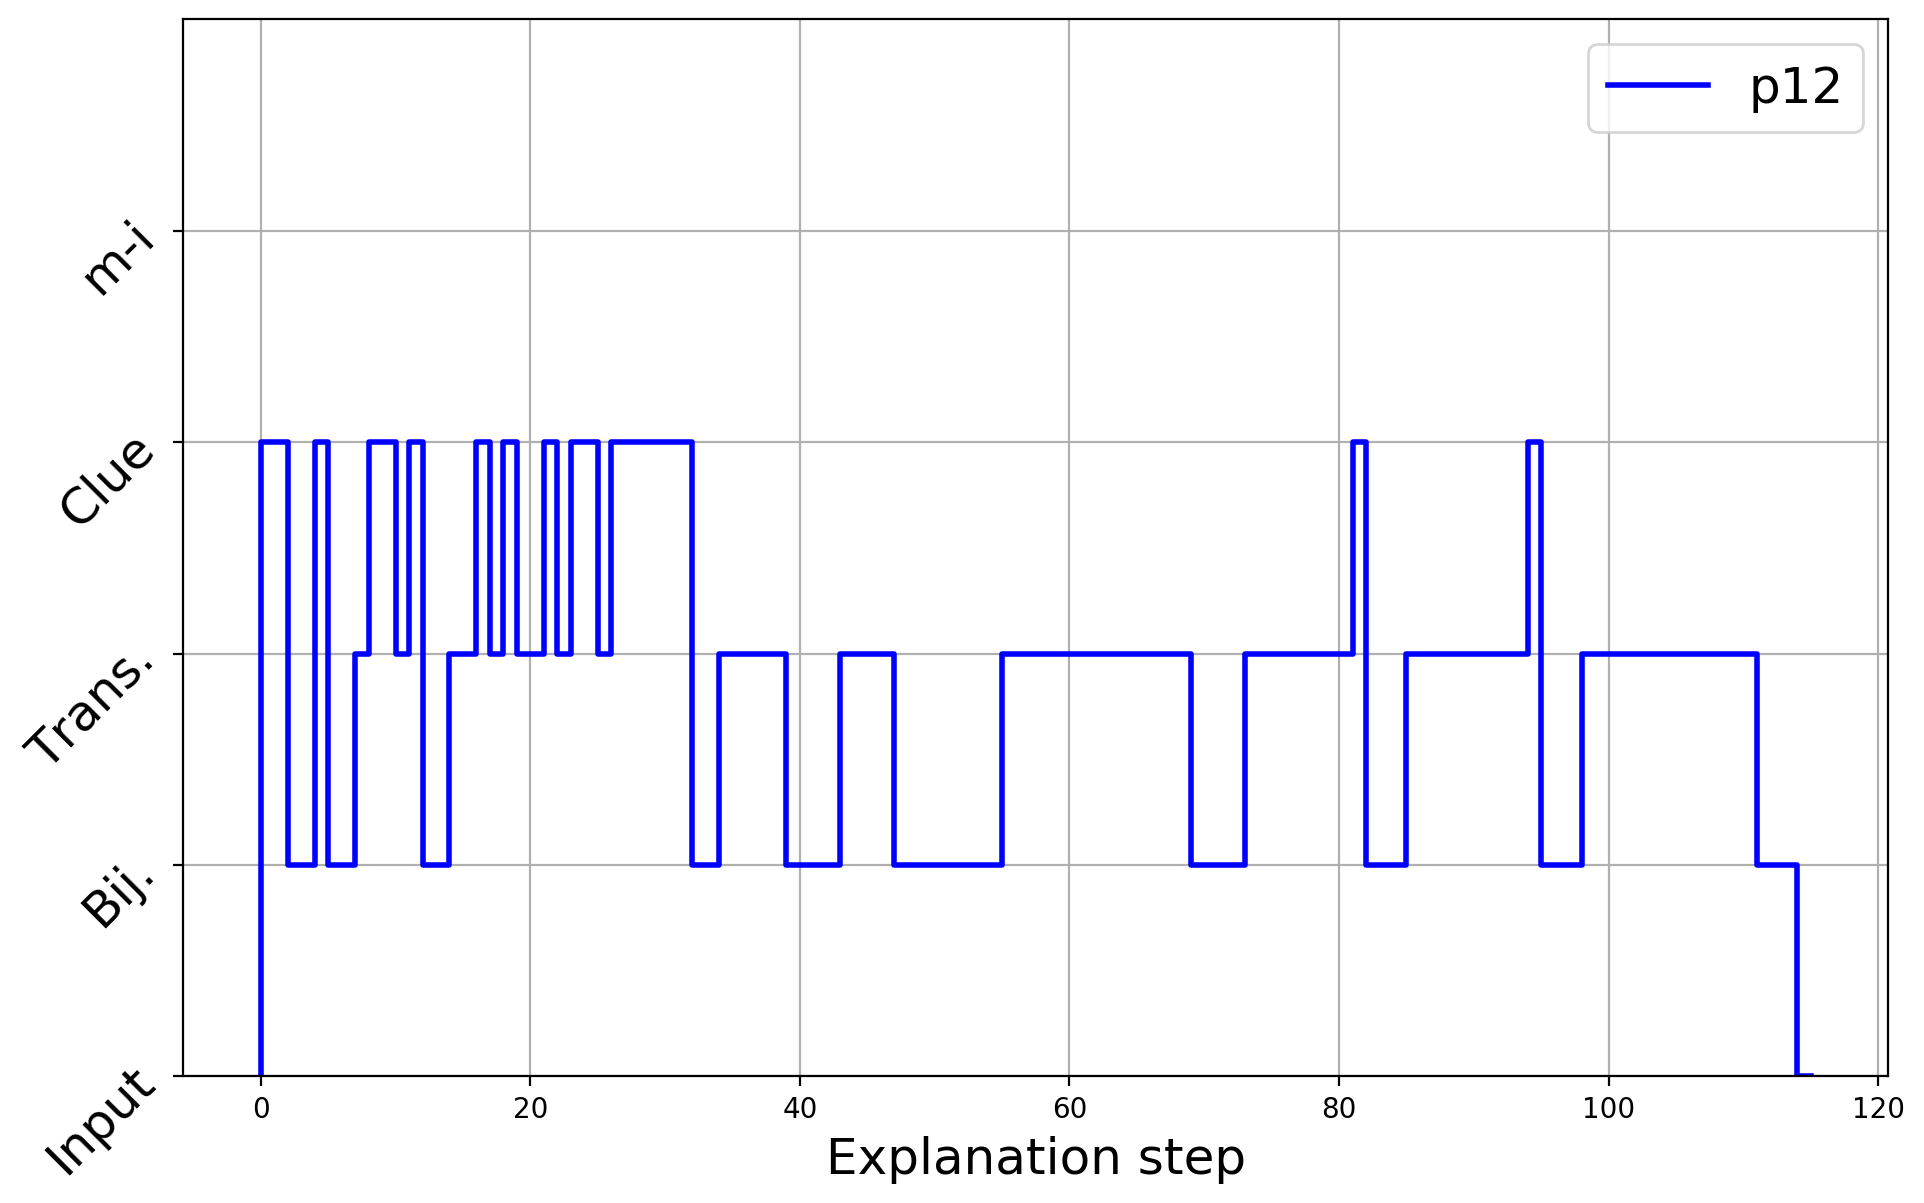
\includegraphics[width=0.49\linewidth]{figures/plot_cost_steps_p12}
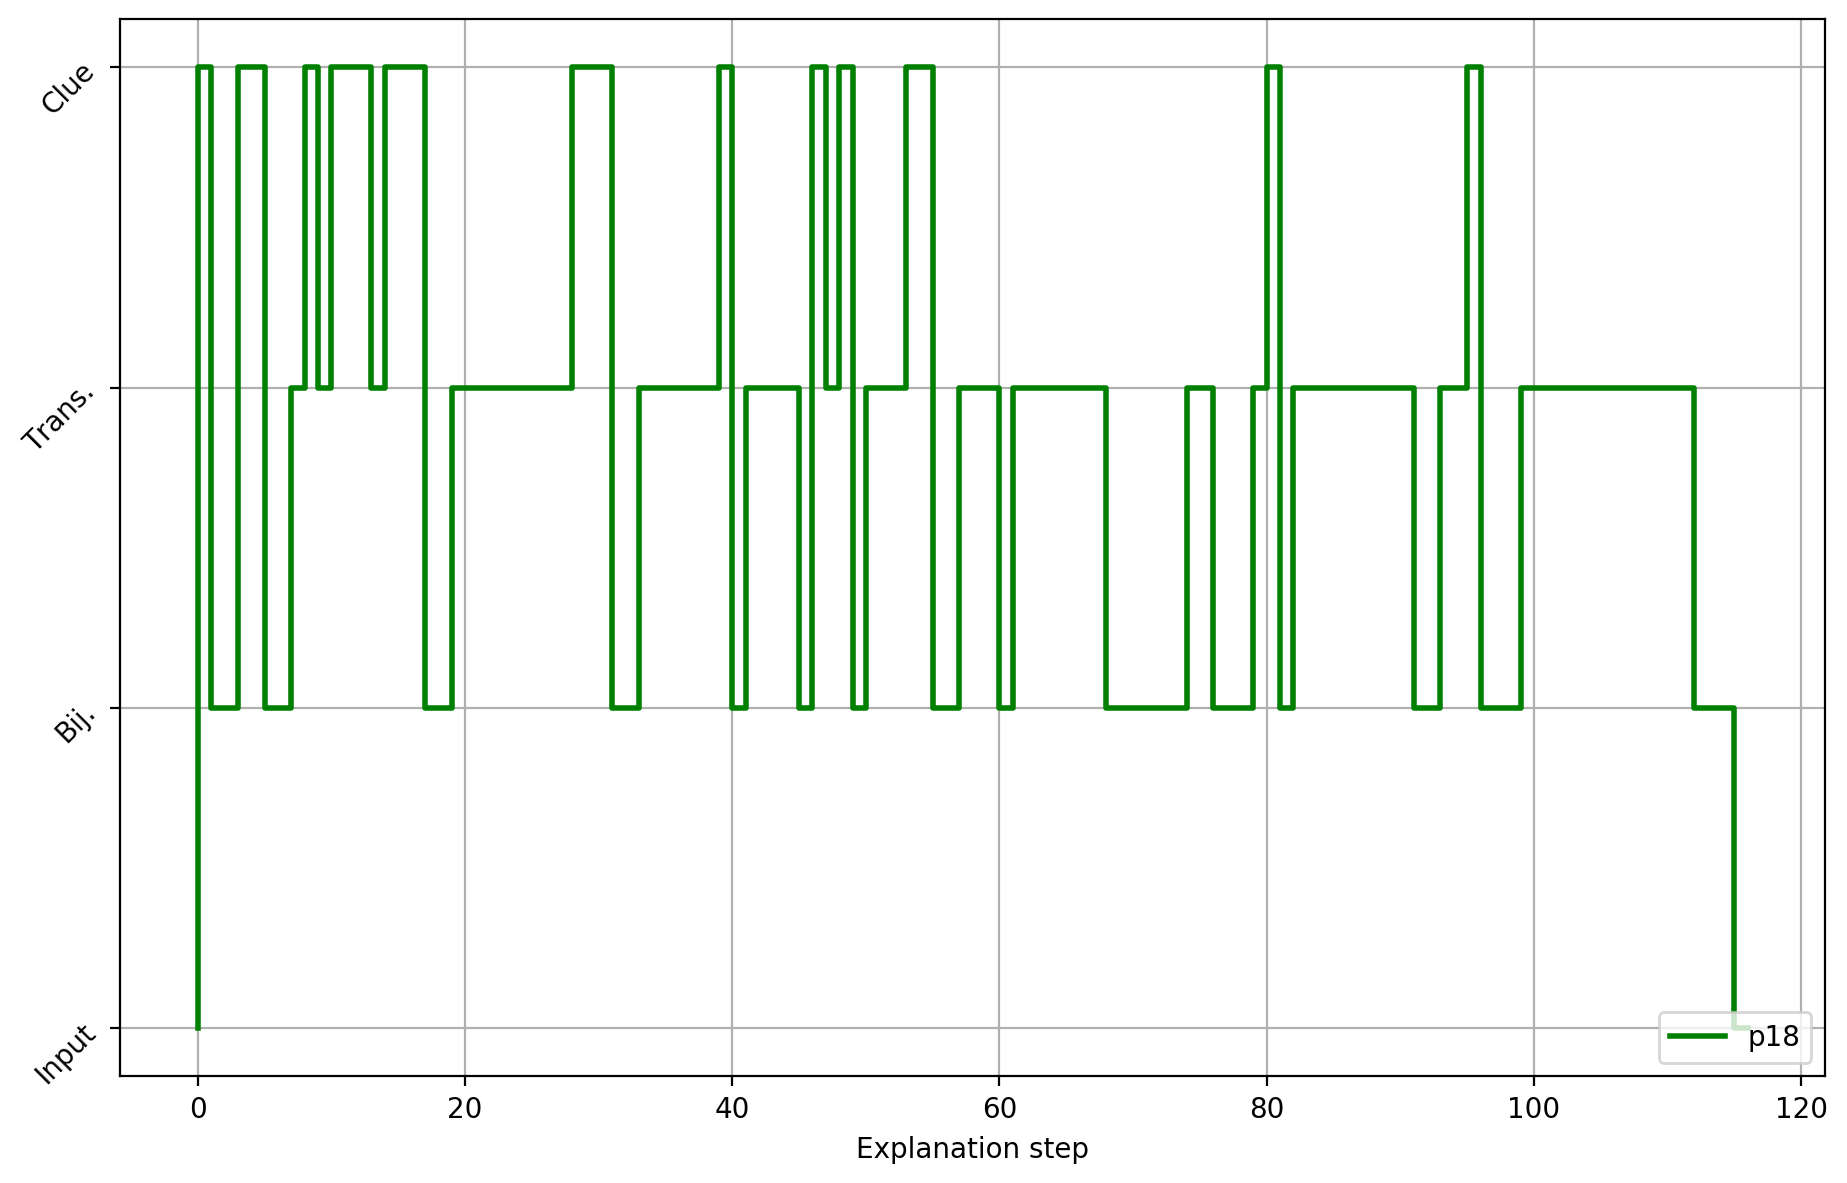
\includegraphics[width=0.49\linewidth]{figures/plot_cost_steps_p18}
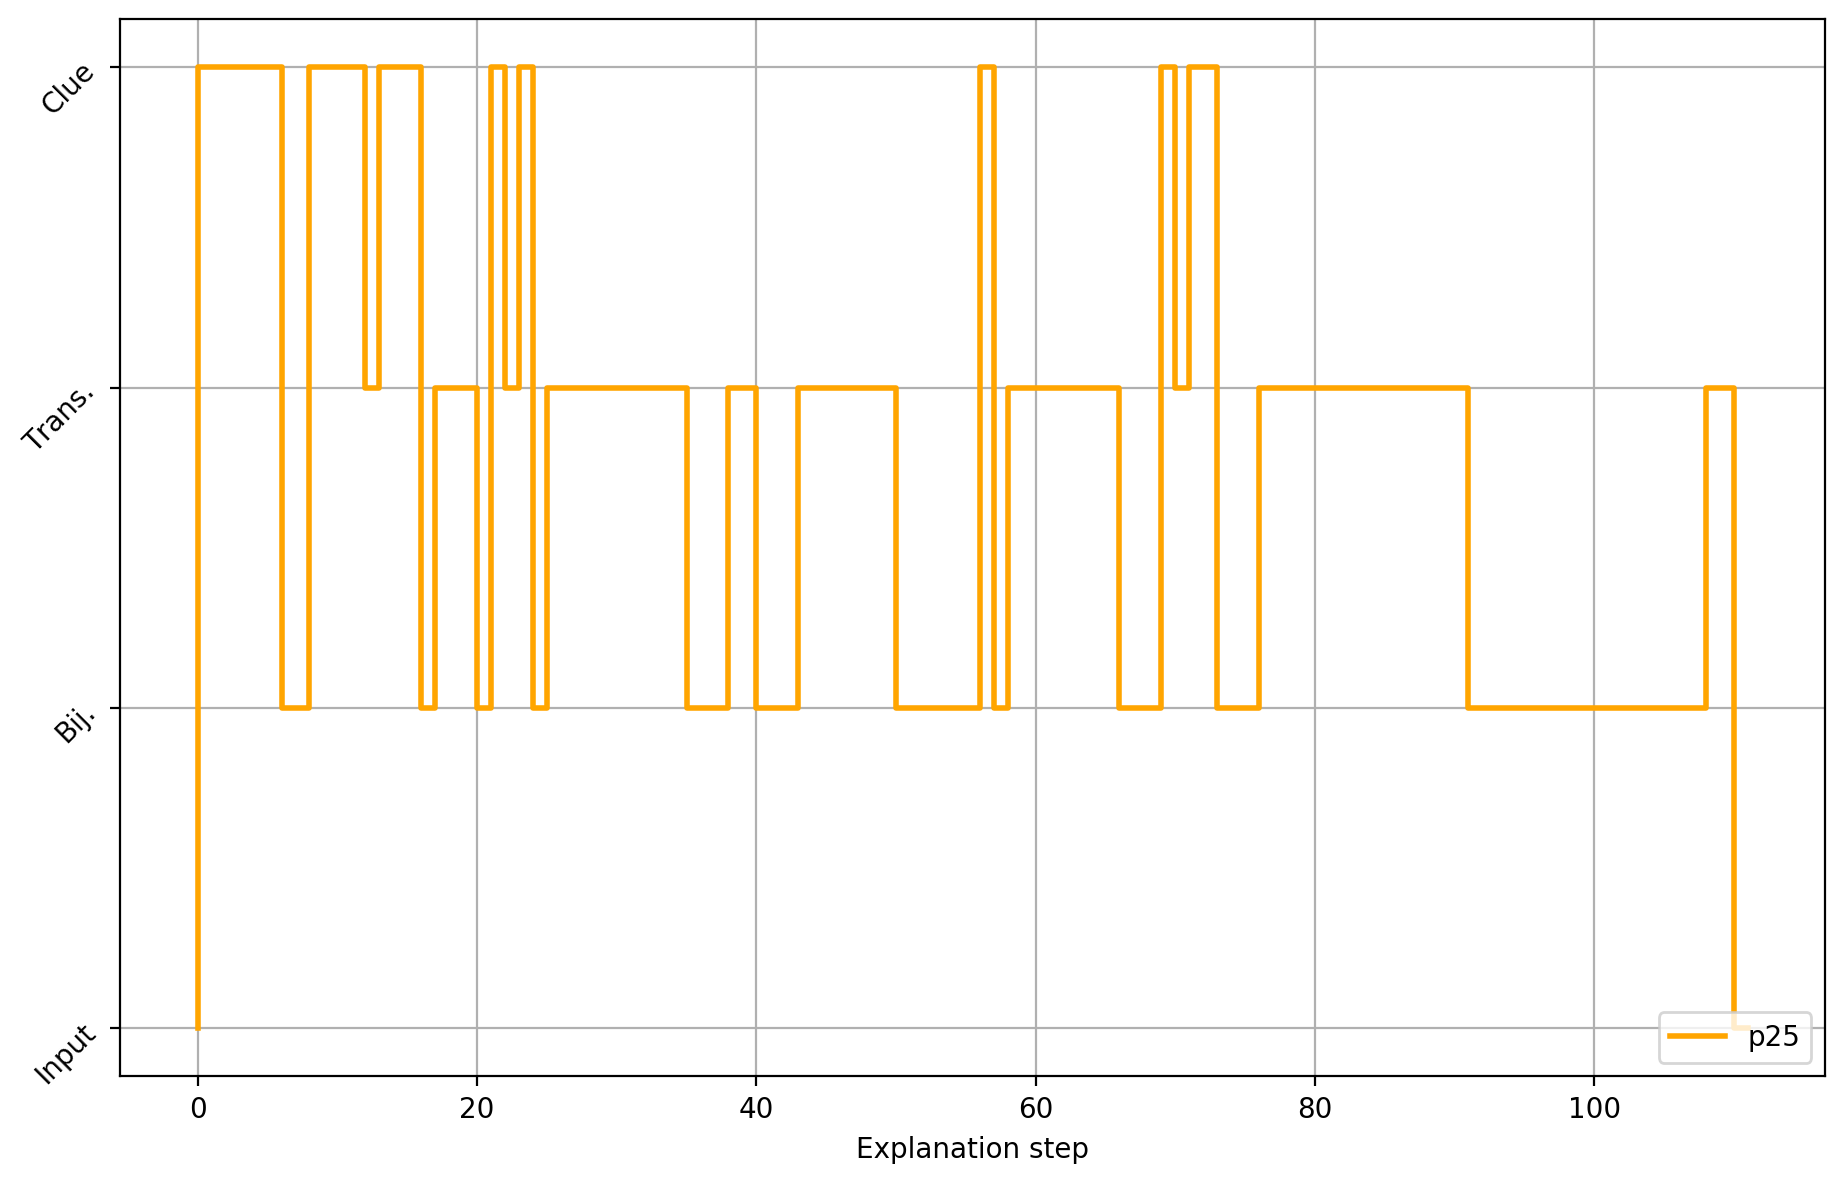
\includegraphics[width=0.49\linewidth]{figures/plot_cost_steps_p25}
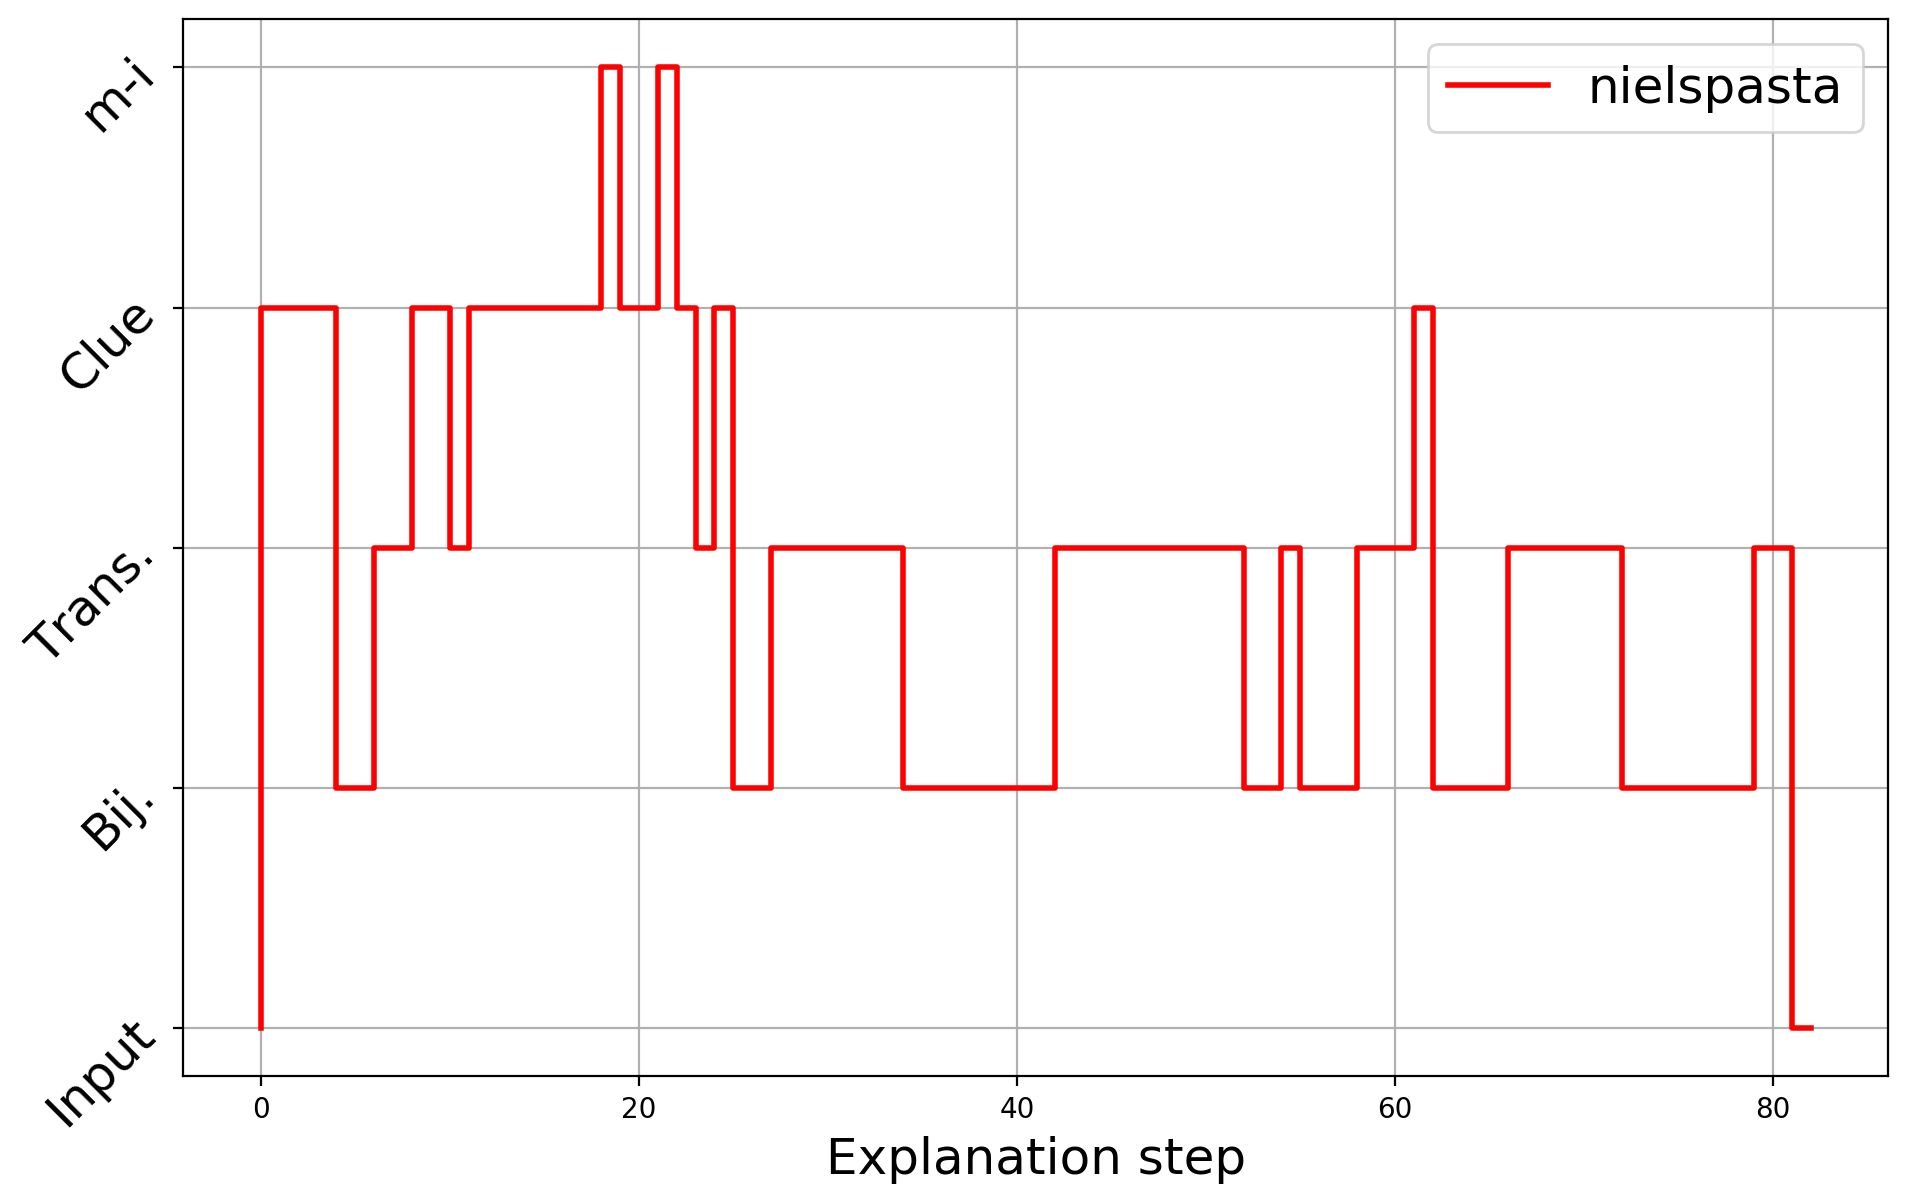
\includegraphics[width=0.49\linewidth]{figures/plot_cost_steps_nielspasta}
\caption{Type of constraints used in each step}
\label{fig:steps}
\end{figure}

\myparagraph{3. Explanation size.}
Our cost-function is constructed to favor few (if any) clues and constraints in the explanations, and few previously derived facts $|E|$. Table~\ref{table:sequence_leve} shows the average number of facts used per explanation. We also show the average number of facts used when using only bijectivity or transitivity, or when a clue is used.

We can observe that the average number of facts used is indeed low, less than two. Further more, the breakdown shows that bijectivity typically uses more facts, e.g. it uses three 'negative' facts in one row to infer a 'positive' fact, as in Figure~\ref{fig:zebrascreen} or it uses one 'positive' fact to infer three negative facts. Note that for such an intuitive constraint, the number of facts used does not matter much. Transitivity, by nature, always uses two previously derived facts. Finally, when looking at the number of facts used together with a clue we can see that our approach succesfully finds small explanations: a number of clues (the trivial ones) use no facts, while most use 1 fact and rarely 2 facts are needed. %\tias{Check when new table arrives}.
The exception is again the difficult pasta puzzle, in which 25\% of the time more than 2 facts are used.

\tias{Ideal table:}

\begin{table}
	\centering
	\resizebox{\columnwidth}{!}{%
		\begin{tabular}{l|c|ccc|cccc} 
		    & \multicolumn{4}{c|}{\bf avg. facts} & \multicolumn{4}{c}{\bf \% of clue expl. with facts} \\
			\textbf{p} & \textbf{all} & \textbf{Bij.} & \textbf{Trans.} & \textbf{Clues} & \textbf{0 facts} & \textbf{1 fact} & \textbf{2 facts} & \textbf{$>$2 facts}\\ 
\hline
	%p5
	1 & 1.82 & 0.52 & 2.0 & 2.37 &66.6\% &28.5\% &0.0\% &4.7\% \\ 
	%p16
	2 & 1.80 & 0.61 & 2.0 & 2.38 &47.8\% &47.8\% &0.0\% &4.3\% \\ 
	%p12
	3 & 1.83 & 0.31 & 2.0 & 2.45 &78.9\% &15.7\% &0.0\% &5.2\% \\ 
	%p18
	4 & 1.85 & 0.45 & 2.0 & 2.50 &70.0\% &15.0\% &15.0\% &0.0\% \\ 
	%p19
	5 & 1.87 & 0.40 & 2.0 & 2.60 &65.0\% &30.0\% &5.0\% &0.0\% \\ 
	%p20
	6 & 1.82 & 0.29 & 2.0 & 2.35 &76.4\% &17.6\% &5.8\% &0.0\% \\ 
	%p25
	7 & 1.93 & 0.73 & 2.0 & 2.46 &57.8\% &26.3\% &5.2\% &10.5\% \\ 
	%p93
	8 & 1.84 & 0.18 & 2.0 & 2.57 &81.8\% &18.1\% &0.0\% &0.0\% \\ 
	%pasta
	p & 1.76 & 1.05 & 2.0 & 2.07 &60.0\% &15.0\% &0.0\% &25.0\% \\ 
		\end{tabular} 
	}
	\caption{Puzzle explanation cost based on the cost function $f(I, C)$ and statistics on puzzle constraints}
	\label{table:sequence_leve}
\end{table}



			pasta & 4 & 5 & 150 & 82 & 34.15 & 40.24 & 21.95 & 2.44 & 0\\ 


%\paragraph{Bonus. How well does it compare to human solving process ?} 

% TODO Compare with the tutorial puzzle of logicgridpuzzles.com? Ideally, a small human evaluation (e.g. ask people to solve a 3-with-3 puzzle and note the order of derivations and clues used, compare this 'ranking' to our ranking, discuss some differences.



\section{Discussion and conclusions}
We presented... it is awesome.

Higher order? How to deal with search; optimisation? learning the cost-function based on traces of users.


\tias{Should this paragraph be here? It seems to undermine our proposed approach... maybe to future work?}
In principle our problem of finding subset-minimal (or even, see the next paragarph, cost-optimal) justifications could be solved by specifying it in such a way in second-order logic and subsequently finding models for it, e.g. by a reduction to QBF \cite{kr/BogaertsTS16,kr/vanderHallenJ18}. 
However, since this is already an $\exists\forall\exists SO$ specification, we expect this approach not be feasible (this expectation remains to be verified in future work). 

\bibliographystyle{ecai}
\bibliography{refs}
\end{document}
%%%%%%%%%%%%%%%%%%%%%%%%%%%%%%%%%%%%%%%%%%%%%%%%%%%%%%%%%%%%%%%%%%%%%%
